
\chapter{Neural Networks}

In this chapter, we'll briefly discuss some concepts on \textit{Neural Networks} (or NNs) and a little bit of \textit{Machine Learning}. NNs will later be used as a function approximator in the Policy Gradient chapter and was also a subject of study during the making of this work.

\section{Machine Learning}
Nowadays, as the Internet continues to expand, we have more and more information available and stored everyday. Due to that large volume of data, analyzing it and extracting meaningful information has become a task increasingly difficult for humans to perform. From that challenge, the concept of \textit{Machine Learning} arises.

Machine learning can be defined as a set of techniques (or algorithms) that allows for a computer program to extract information, identify paterns and relationships in large amounts of data, in such a way a human cannot.

According to \cite{Mitchell}, \textit{"A computer program is said to learn from experience $E$ with respect to some class of tasks $T$ and performance measure $P$ if its performance at tasks in $T$, as measured by $P$, improves with experience $E$"}.

\cite{Goodfellow-et-al-2016} broke machine learning down to 3 main paradigms:
\begin{itemize}
    \item In \textbf{Supervised Learning}, we have a dataset containing features, but each example is also associated with a \textit{label} or \textit{target}. For example, a dataset containing emails labeled as \textbf{spam} or \textbf{not spam}. A supervised learning algorithm can study this dataset and learn to classify whether an email is a spam or not.
    \item In \textbf{Unsupervised Learning}, we have a dataset containing many features, but no labels. Then, the goal is to learn useful properties of the structure of this dataset. In the context of deep learning, we usually want to learn the entire probability distribution that generated the dataset. Some other unsupervised learning algorithms perform other roles, like clustering, which consists of dividing the dataset into clusters of similar data.
    \item Then, there's \textbf{Reinforcement Learning}, where we don't have a fixed dataset. Instead, RL algorithms interact with the environment, forming a feedback loop between the learning system and what it has experienced.
\end{itemize}

\section{Neural Networks}
Neural Networks are a set of machine learning algorithms, whose structure is strongly related with the structure of the human brain. 
\begin{figure}[H]
    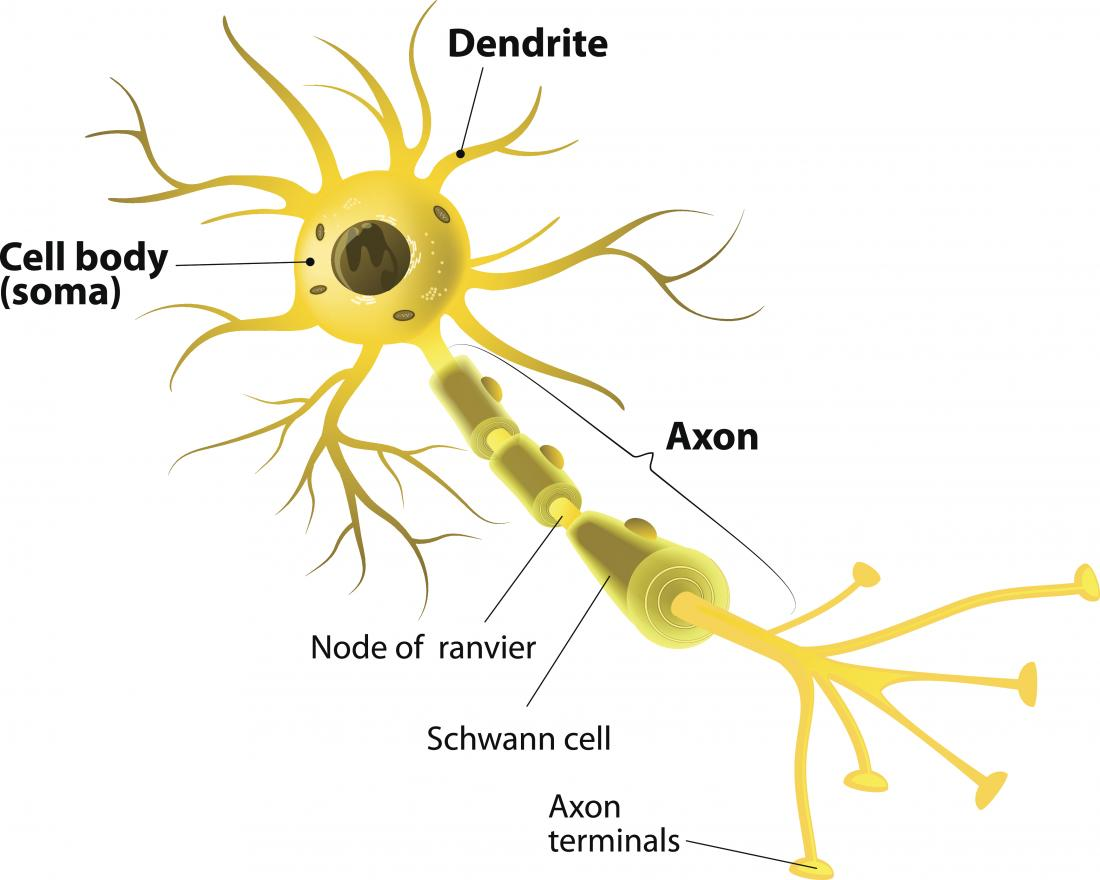
\includegraphics[width=\textwidth]{neuron-diagram}
    \caption{Source: \href{https://www.medicalnewstoday.com/articles/320289}{MedicalNewsToday}}
\end{figure}
The main structural cells responsible for processing information are divided into 3 main parts:
\begin{itemize}
    \item \textbf{Dendrites:} filaments responsible for receiving and transporting stimulus coming from the environment or other cells of the body.
    \item \textbf{Body cell:} processes the information gathered by the dendrites.
    \item \textbf{Axon:} transmits the nervous impulses generated by the cell body to the other cells through the axon terminals.
\end{itemize}
In summary, upon receiving stimuli, the cell body processes those signals and if the result exceeds a certain threshold value, the neuron fires a nerve impulse indicating it reacted to the input signals, which are further transmitted by other neurons to other neurons or cells.

The human brain processes information processes in order $10^{-3}$ seconds, having a network of about 10 billion neurons densely connected, making it a huge, complex and efficient processing powerhouse, performing tasks like recognizing images and audios better than any machine. In an attempt to recreate a system that was able to operate like a human brain, the concept or \textit{Artificial Neural Networks} was idealized.

\cite{haykin2009neural} cites the following useful properties and capabilities:
\begin{itemize}
    \item \textbf{Nonlinearity:} an artificial neuron can be linear or nonlinear. Therefore, a neural network, made up of an interconnection of nonlinear neurons, is itself nonlinear. Nonlinearity is a highly important property, particularly if the underlying physical mechanism responsible for generation of the input signal (e.g., speech signal) is inherently nonlinear.
    \item \textbf{I/O Mapping:} neural networks perform very well in supervised learning tasks, where we have labeled data. Each piece of data is used to update the synaptic bias of the network such that the difference between the expected output and the actual output is minimized.
    \item \textbf{Adaptivity:} neural networks have the capability to adapt their synaptic weights to changes in the surrounding environment. 
    \item \textbf{Evidential Response:} in particular, a neural network trained to operate in a specific environment can be easily retrained to deal with minor changes in the operating environmental conditions.
    \item \textbf{Contextual Information:} in the context of pattern classification, a neural network can be designed to provide information not only about which particular pattern to select, but also about the confidence in the decision made. This latter information may be used to reject ambiguous patterns, should they arise, and thereby improve the classification performance of the network.
    \item \textbf{Uniformity of Analysis and Design:} neural networks enjoy universality as information processors, in a sense that the same notation is used in all domains involving the application of neural networks, making it possible to share techniques and theories between models with different purposes.
    \item \textbf{Neurobiological Analogy:} the design of a neural network is motivated by analogy with the brain, which is a living proof that parallel processing is not only physically possible, but also fast and powerful.
\end{itemize}

\section{Perceptron}
In order to create a model that would function similarly to a human brain, the psychologist and neurobiologist Frank Rosenblatt proposed the \textit{perceptron} model. In his words, "a probabilistic model for information storage and organization in the brain" \cite{rosenblatt:perceptron}.
\begin{figure}[H]
    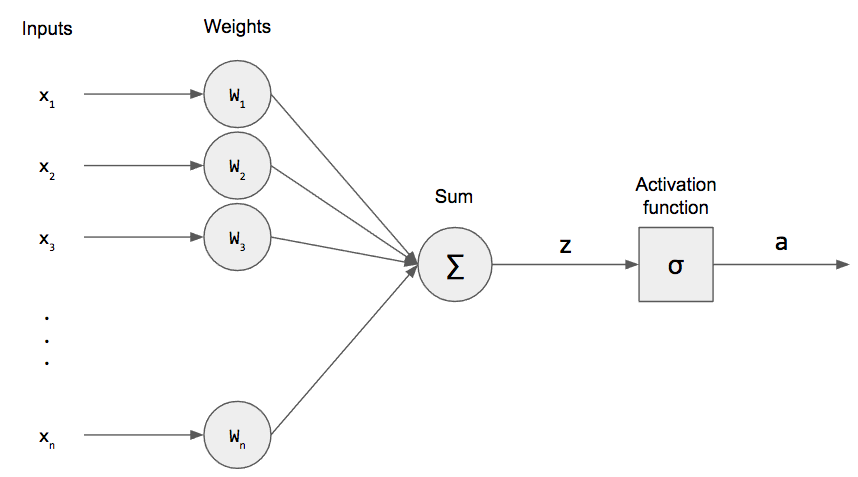
\includegraphics[width=\textwidth]{perceptron}
    \caption{Source: \href{https://medium.com/@stanleydukor/neural-representation-of-and-or-not-xor-and-xnor-logic-gates-perceptron-algorithm-b0275375fea1}{Medium}}
\end{figure}
In this artificial neuron, we have the following structures:
\begin{itemize}
    \item An input vector $x \in \mathbb{R}^n$
    \item The synaptic weights $w \in \mathbb{R}^n$ responsible for weighing the values from the input vector. Large and positive values indicate higher relevance. Conversely, small and negative values indicate lower relevance.
    \item A bias $b \in \mathbb{R}$, which can be interpreted as how easily a neuron is activated.
    \item A linear combinator $\Sigma$ weighing the input signals into a single scalar value:
    \[
        z = \Sigma(x) = \sum^{i=1}_{n}w_i x_i + b   
    \]
    \item An activation function $\phi \colon \mathbb{R} \to \mathbb{R}$ mapping the weighted sum $z$ to an output $\phi(z)$.
\end{itemize}
In general, given $w \in \mathbb{R}^n$ and $b \in \mathbb{R}$, the perceptron model can be defined as a function $h \colon \mathbb{R}^n \to \mathbb{R}$ such that
\[
    h(x \mid w, b) = \phi(w^Tx + b)    
\]

From the perceptron, multiple models have been derived, but we are particularly interested in a specific \textit{feed-forward} neural network, called \textit{multilayer perceptron}.

\section{Multilayer Perceptron}
In a multilayer perceptron, the perceptrons (neurons) are stacked in mutiple layers in such a way that every node on each layer is connected to all other nodes on the next layer, without any cycles, characterizing the \textit{feed-forward} nature of the model.

The first layer is the input layer, and its units take the values of the input vector. The last layer is the output layer, and it has one unit for each value the network outputs. In the context of classification, it could have a single unit in the case of binary classifiation, or $K$ units in the case of $K$-class classification. All the layers in between these are called hidden layers. It's called hidden because we don't know ahead of time what these units should compute, and this needs to be discovered during learning \cite{grosse2021}.

\begin{figure}[H]
    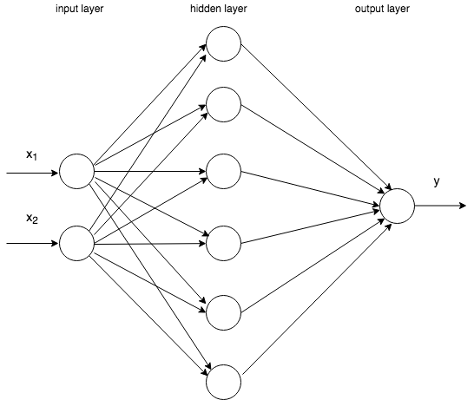
\includegraphics[width=\textwidth]{mlp}
    \caption{Source: \href{https://kinder-chen.medium.com/multilayer-perceptron-55bb39a08133}{Medium}}
\end{figure}
Such as the perceptron, the MLP can also be defined as a function. Denote by $h_i^{(l)}$ the $i$-th unit in the $l$-th hidden layer and by $y$ the output unit. Note that each unit has its own bias, and there's a weight for every pair of units in two consecutive layers. Therefore, the network's computation can be expressed as:
\begin{align}
    h_i^{(1)} &= \phi^{(1)} \left(\sum_j w_{ij}^{(1)}x_j + b_i^{(1)}\right) \nonumber \\
    h_i^{(2)} &= \phi^{(2)} \left(\sum_j w_{ij}^{(2)}h_j^{(1)} + b_i^{(2)}\right) \\
    y_i &= \phi^{(3)} \left(\sum_j w_{ij}^{(3)}h_j^{(2)} + b_i^{(3)}\right) \nonumber
\end{align}

An important result for MLP models is the Universal Approximation Theorem \cite{journals/mcss/Cybenko89}:
\begin{theorem}{Universal Approximation Theorem}{}
    Let $\sigma: \mathbb{R} \rightarrow \mathbb{R}$ be a continuous, bounded, non-constant and monotonically decreasing function. Let $I_{n}=[0,1]^{n}$ be the n-dimensional hypercube and $C\left(I_{n}\right)$ the space of continuous functions in $I_{n}$. Then, given $f \in C\left(I_{n}\right)$ independent of $\sigma$ and $\epsilon>0$, there exists $N \in \mathbb{N}, w_{i} \in \mathbb{R}^{n}, b_{i} \in \mathbb{R}$ and $\alpha_{i} \in \mathbb{R}$, where $i=1, \ldots, N$ such that 
    \[
    \begin{aligned}
    &F(x)=\sum_{i=1}^{N} \alpha_{i} \sigma\left(w_{i} . x+b_{i}\right), \\
    &|F(x)-f(x)|<\epsilon,
    \end{aligned}
    \]
    for all $x \in I_{n}$.
\end{theorem}
The theorem estabilishes that for any continuous function $f$ on a compact subset of $I_n$ can be approximated by a feed-forward neural network with only one hidden layer and finite number of units.

It's important to note that this doesn't imply that one neural network can accurately approximate any arbitrary continuous function under any circumstances. It is required that the neural network and its parameters (number of hidden units, number of learning iterations etc.) be adjusted for each unique function. Then, with the right parameters, it is possible to achieve any desired accuracy $\epsilon$.

Cybenko proved the theorem specifically for \textit{sigmoid} activation functions $Sigmoid(x)=\dfrac{1}{1+e^{-x}}$
\begin{figure}[H]
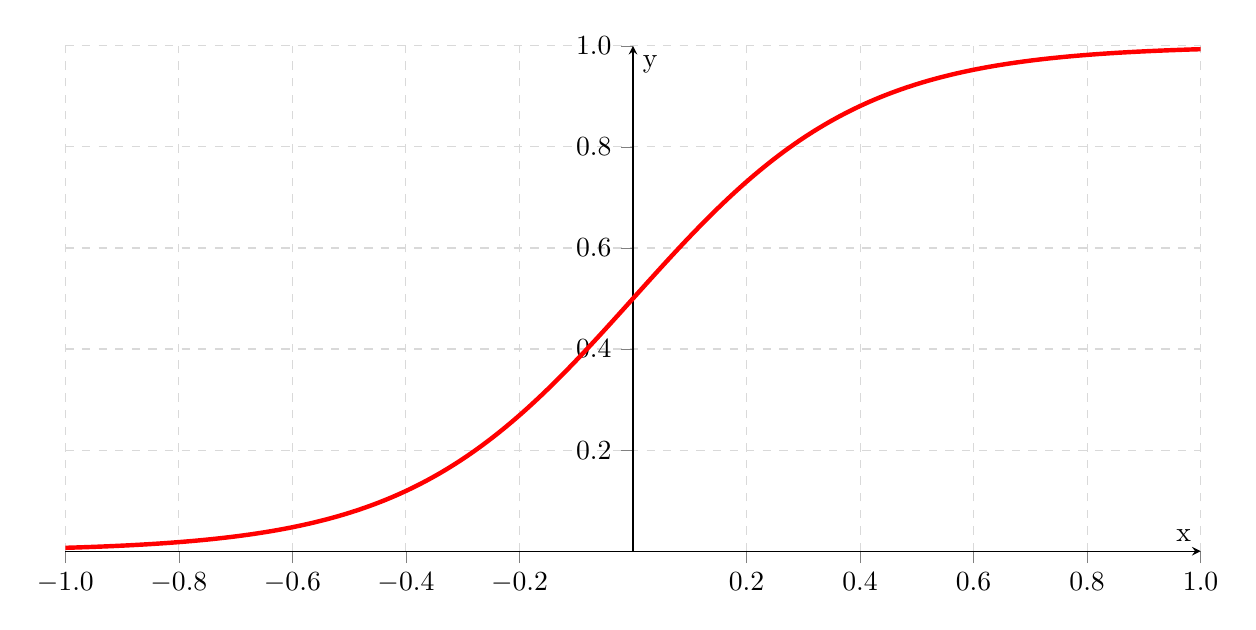
\begin{tikzpicture}
    \begin{axis}[
    	legend pos=north west,
        axis x line=middle,
        axis y line=middle,
        x tick label style={/pgf/number format/fixed,
                            /pgf/number format/fixed zerofill,
                            /pgf/number format/precision=1},
        y tick label style={/pgf/number format/fixed,
                            /pgf/number format/fixed zerofill,
                            /pgf/number format/precision=1},
        grid = major,
        width=16cm,
        height=8cm,
        grid style={dashed, gray!30},
        xmin=-1,     % start the diagram at this x-coordinate
        xmax= 1,    % end   the diagram at this x-coordinate
        ymin= 0,     % start the diagram at this y-coordinate
        ymax= 1,   % end   the diagram at this y-coordinate
        %axis background/.style={fill=white},
        xlabel=x,
        ylabel=y,
        tick align=outside,
        enlargelimits=false]
      % plot the stirling-formulae
      \addplot[domain=-1:1, red, ultra thick,samples=500] {1/(1+exp(-5*x))};
    \end{axis}
\end{tikzpicture}
\caption{Graph for the Sigmoid function.}
\end{figure}
Other activation functions have also been shown to satisfy the theorem, such as:
\begin{itemize}
    \item Hyperbolic Tangent
    \[
        \phi(z) = \frac{2}{1+e^{-2z}}-1 = 2Sigmoid(2z) - 1    
    \]
    \item Softsign
    \[
        \phi(z) = \frac{z}{1+|z|}
    \]
\end{itemize}
Recently, other activation functions have also proven to be very effective as approximators, but don't satisfy the theorem, since they're not bounded:
\begin{itemize}
    \item Rectified Linear Unit (ReLU)
    \[
        \phi(z) = \max\{0, z\}    
    \]
    \item Softplus
    \[
        \phi(z) = ln(e^z+1)
    \]
    \item Exponential Linear Unit (ELU)
    \begin{equation*}
        \phi(z)=
            \begin{cases}
                \alpha(e^z-1) & \text{if } z < 0 \\
                z & \text{if } z \geq 0
            \end{cases}
    \end{equation*}
    for $\alpha \in \mathbb{R}$.
\end{itemize}

The theorem also has an extension for the case with multiple hidden layers and outputs, but will not be addressed here.